% Ubah kalimat sesuai dengan judul dari bab ini
\chapter{TINJAUAN PUSTAKA}
\vspace{4ex}

% Pengaturan ukuran indentasi
\setlength{\parindent}{7ex}

% Ubah konten-konten berikut sesuai dengan yang ingin diisi pada bab ini

\section{Roket Luar Angkasa}
\vspace{1ex}

% Contoh input gambar dengan format *.jpg
\begin{figure} [ht] \centering
  % Nama dari file gambar yang diinputkan
	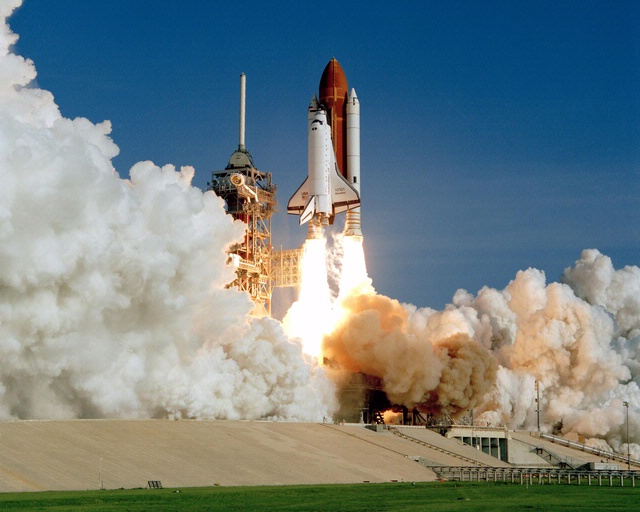
\includegraphics[scale=0.45]{gambar/space-shuttle.jpg}
  % Keterangan gambar yang diinputkan
	\caption{Peluncuran Pesawat Luar Angkasa \emph{Discovery}}
  % Label referensi dari gambar yang diinputkan
	\label{fig:spaceShuttle}
\end{figure}

Roket luar angkasa merupakan \lipsum[1]
\vspace{0.5ex}

% Contoh penggunaan referensi dari gambar yang diinputkan
\emph{Discovery} \ref{fig:spaceShuttle} merupakan \lipsum[2]

Beberapa keunggulan dari \lipsum[3][1-2] adalah:
\vspace{0.5ex}

\begin{enumerate}[nolistsep]

  \item Mempermudah \lipsum[1][1-2]
  \vspace{0.5ex}

  \item \lipsum[1][3-4]
  \vspace{0.5ex}

\end{enumerate}
\vspace{0.5ex}

\section{Gravitasi}
\vspace{1ex}

Gravitasi merupakan \lipsum[1]
\vspace{0.5ex}

\subsection{Hukum Newton}
\vspace{1ex}

% Contoh penggunaan referensi dari pustaka
Newton pernah merumuskan \citep{newtonLaw} bahwa \lipsum[2]
% Contoh penggunaan referensi dari persamaan
Kemudian menjadi persamaan seperti pada persamaan \ref{eq:hukumPertama}.
\vspace{0.5ex}

% Contoh pembuatan persamaan
\begin{equation}
  % Label referensi dari persamaan yang dibuat
  \label{eq:hukumPertama}
  % Baris kode persamaan yang dibuat
  \sum \mathbf{F} = 0\; \Leftrightarrow\; \frac{\mathrm{d} \mathbf{v} }{\mathrm{d}t} = 0.
\end{equation}
\vspace{0.5ex}

\subsection{Anti Gravitasi}
\vspace{1ex}

Anti gravitasi sendiri merupakan \lipsum[3]
\vspace{0.5ex}